\documentclass[english]{article}

\usepackage{graphicx}
\usepackage{grffile}
\usepackage{babel}
\usepackage{float}

\textwidth = 426pt
\oddsidemargin = 17pt

\author{
    Jita, Hlengekile\\
    \texttt{u14077893}
    \and
    Moodley, Joshua\\
    \texttt{u14152152}
    \and
    Kazadi, Dieumerci\\
    \texttt{u16353383}
    \and
    Nell, Stephan\\
    \texttt{u15124861}
    \and
    Rayner, Peter\\
    \texttt{u14001757}
    \and
    Van Hattum, Jason\\
    \texttt{u15027458}
    \and
    Schuld, Bernhard\\
    \texttt{u10297902}
}

\title{Architectural Requirements Specification\\
    for the NavUP System\\
    }
\date{\today}
\graphicspath{{Images/}}

\begin{document}
    \fboxsep=2mm

    \maketitle
    \begin{figure}[!t]
        
\includegraphics{up_logo.png}
    \end{figure}
    \pagenumbering{gobble}
    \newpage

    \tableofcontents
    \newpage

    \pagenumbering{arabic}


    \section{Introduction}
        This document will serve to outline the architectural requirements, constraints and design for the NavUP system. The general pattern that the system will be built around will also be discussed.\\
        \\
        In addition, the subsystems will be descried along with their planned implementation, accompanied by relevant diagrams. With regards to the subsystems, focus will be put onto designing the subsystems to be modular and loosely coupled in such a way that the system can be deployed with a minimal set of subsystems, and each subsystem can be changed without affecting the others.\\
        \\
        The modules that the document will outline are:
        \begin{itemize}
            \item Data.
            \item Users.
            \item Navigation.
            \item Surveillance.
        \end{itemize}

    \section{Overall System Design}
        \subsection{Architecture}
        The system will be designed using the \textbf{n-tier} architecture, where the system is divided into multiple layers, and information is passed from one layer to another. The direction of information transfer is described in further detail in our deployment diagram.

       \subsection{Deployment}
            \begin{figure}[H]
            \centering              
            \centerline{\fbox{\includegraphics[scale=0.2]{Deployment-Diagram.png}}}
            \caption{Deployment Diagram}
        \end{figure}

    % ----- USERS ----- %
    \newpage
    \section{Users}
        The Users module is responsible for the management of NavUP's users. There will be 3 categories of users of the system, Guest users, which will be able to access public services without having to be logged in. Registered users, which will in addition to the public services will be able to store profile information necessary for other activities provided by the system and Admin users which will have the additional ability to manage the users of the system.
        
        In the figure below, is a use case diagram that shows how each user will be able to make use of the Users module and what functionality will be included in order to achieve the use cases.
        \begin{figure}[H]
            \centering              \centerline{\fbox{\includegraphics[scale=0.5]{Users Use Case Diagram.png}}}
            \caption{Use Case Diagram - Users Module}
        \end{figure}
        
        In the figure below is a class diagram that shows the classes of the Users subsystem.
        \begin{figure}[H]
            \centering              \centerline{\fbox{\includegraphics[scale=0.6]{UsersClassDiagram.png}}}
            \caption{Class Diagram - Users Module}
        \end{figure}
        


    % ----- NAVIGATION ----- %
    \newpage
    \section{Navigation}
        \subsection{Description}
            The purpose of the Navigation subsystem is to provide routes to users based on their destination and current location, as well as navigating the users along the route to their destination.\\
            This subsystem will reside almost entirely in the application layer, as it is comprised mostly of decisions related to navigation.

       \subsection{Requirements}
            The Navigation system should be able to:
            \begin{itemize}
                \item Provide a navigable route between two locations to a user on request, taking into account a possible set of preferences.
                \item Navigate a user from waypoint to waypoint until they arrive at their destination.
                \item Detect when a user deviates from their given route and recalculate a new route accordingly.
                \item Persist routes to the database for later use.
            \end{itemize}

        \subsection{Constraints}
            The system must operate under the following constraints:
            \begin{itemize}
                \item Any location data is received from the GIS subsystem, and is assumed to be correct.
                \item The destination is received from the user, and may be impossible to navigate to.
                \item The system has to work with the map as provided by GIS, which may have missing locations or locations that are incorrectly placed.
            \end{itemize}

        \subsection{Design}
            The Navigation system is implemented as 10 classes organised in two well-known design patterns - the Strategy and Memento patterns.

            \subparagraph{Strategy}
            The portion of the system which calculates routes is implemented in such a way that the algorithm can be changed easily by simple adding a class. This is done with the Strategy design pattern - each extra routing algorithm is simply added by adding a new class which inherits from \texttt{RouteAlgorithm}, and overrides the \texttt{calculate()} function. Decompiling each algorithm to a separate class will help with maintaining the code in the future and will reduce the overall complexity of the navigation module.

            \subparagraph{Memento}
            One of the requirements of the system is to save the route. The system will accomplish this by saving the waypoints as they are reached. The Memento design pattern is used here - each waypoint is saved as a \texttt{WaypointMemento} object to the database, which ensures that the state is unchanged when the object is recovered at a later stage.

        \begin{figure}[H]
            \centering              
            \centerline{\fbox{\includegraphics[scale=0.25]{Navigation-Class-Diagram.png}}}
            \caption{Class Diagram - Navigation Module}
        \end{figure}

        \subsection{Implementation Details}
            The system will, for the most part, be composed of a graph. In the graph each node would represent a location, with the links between the nodes representing the paths from location to location. \\
            Navigating from one location-node to another would then simply be a matter of using some shortest-path algorithm to find the path. The algorithm would depend on the user's preferences such as finding the shortest path as opposed to the quickest path, and so on. These algorithms would be interchangeable due to the use of the Strategy pattern. \\
            The nodes would be saved as \textit{Location} objects, and the route calculated by a \texttt{RouteAlgorithm} object.

        \begin{figure}[H]
            \centering              
            \centerline{\fbox{\includegraphics[scale=0.75]{Graph-Navigation.png}}}
            \caption{Example Navigation Graph - Navigation Module}
        \end{figure}

        \begin{figure}[H]
            \centering              
            \centerline{\fbox{\includegraphics[scale=0.45]{Navigation-State-Diagram.png}}}
            \caption{State Diagram - Navigation Module}
        \end{figure}

        \begin{figure}[H]
            \centering              
            \centerline{\fbox{\includegraphics[scale=0.65]{Navigation-Case-Diagram.png}}}
            \caption{Use Case Diagram - Navigation Module}
        \end{figure}

    % ----- DATA ----- %
    \newpage
    \section{Data}
        \subsection{Description}
        The data subsystem is responsible for handling and responding to requests for information, as well as persisting information to a database.
        
        \subsection{Requirements}
        \begin{itemize}
            \item The database should be able to manage a very large amount of concurrent requests.
            \item Data requests should be performed reliably and consistently.
            \item Data should be duplicated (Such as in RAID 5) or backed up for redundancy and performance.
        \end{itemize}
        
        \subsection{Constraints}
        \begin{itemize}
            \item The system has to store data of similar types for consistency.
            \item The system has to make use of the existing UP server infrastructure.
        \end{itemize}
        
        \subsection{Implementation Details}
        The Data subsystem provides the role of Broker in the entire system, in the sense that all requests for information are made through the data subsystem. This allows for low coupling. The actual data system will be implemented as an Iterator, as seen in the class diagram. This is to allow data responses to be accessed without exposing their underlying representation. This promotes component-based development, boosts productivity in data access, and reduces configuration management in the database.\\
        The database used by the Data subsystem will make use of a SQL database in order to be consistent with the existing UP database infrastructure.
        
        \begin{figure}[H]
            \centering              
            \centerline{\includegraphics[scale=0.5]{Data-Case-Diagram.png}}
            \caption{Use Case Diagram - Data Module}
        \end{figure}
        
        \begin{figure}[H]
            \centering              
            \centerline{\fbox{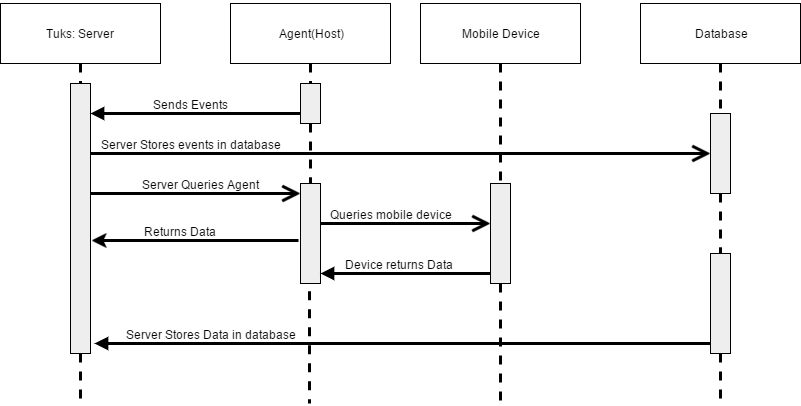
\includegraphics[scale=0.5]{Data-Sequence-Diagram.png}}}
            \caption{Sequence Diagram - Data Module}
        \end{figure} 

        \begin{figure}[H]
            \centering              
            \centerline{\fbox{\includegraphics[scale=0.5]{Data-Activity-Diagram.png}}}
            \caption{Activity Diagram - Data Module}

        \end{figure} 
        
        \begin{figure}[H]
            \centering              
            \centerline{\fbox{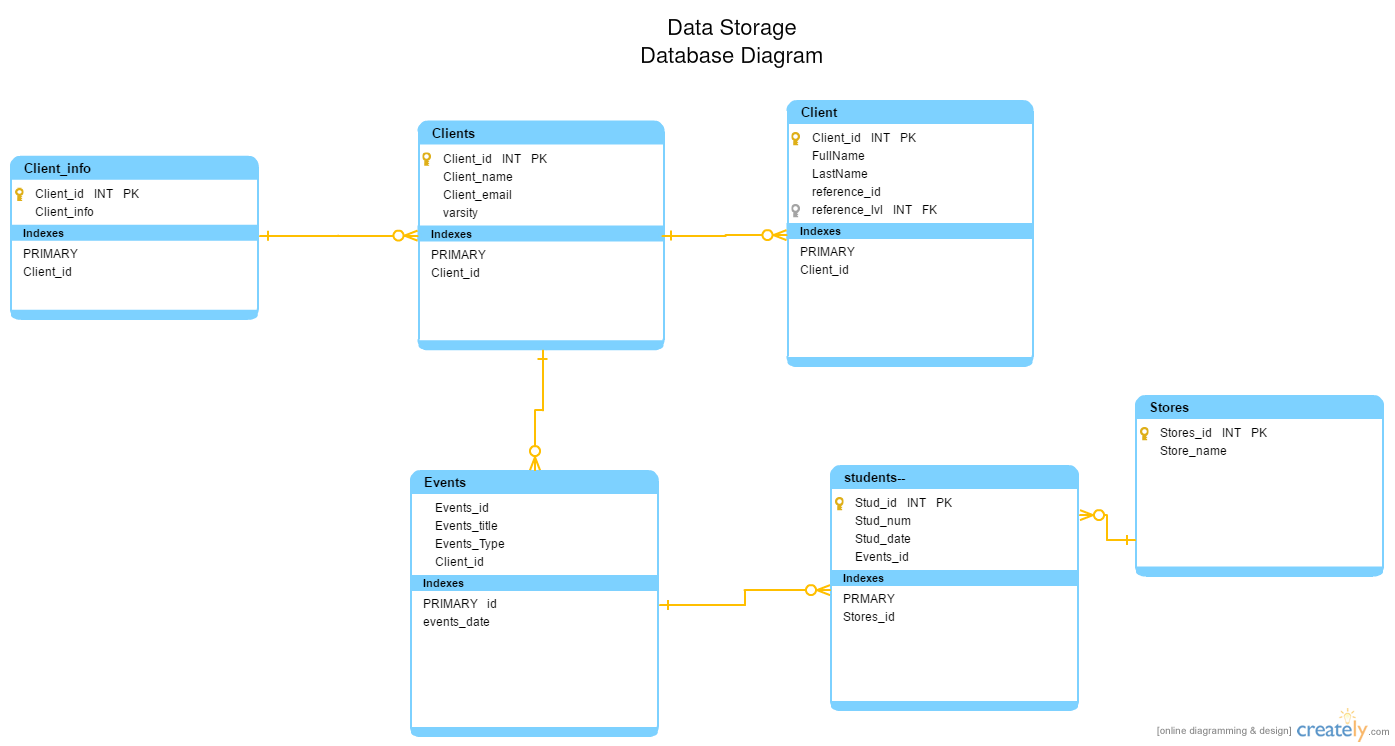
\includegraphics[scale=0.4]{Data-Database-Diagram.png}}}
            \caption{Database Diagram - Data Module}
        \end{figure}     
        
        \begin{figure}[H]
            \centering              
            \centerline{\fbox{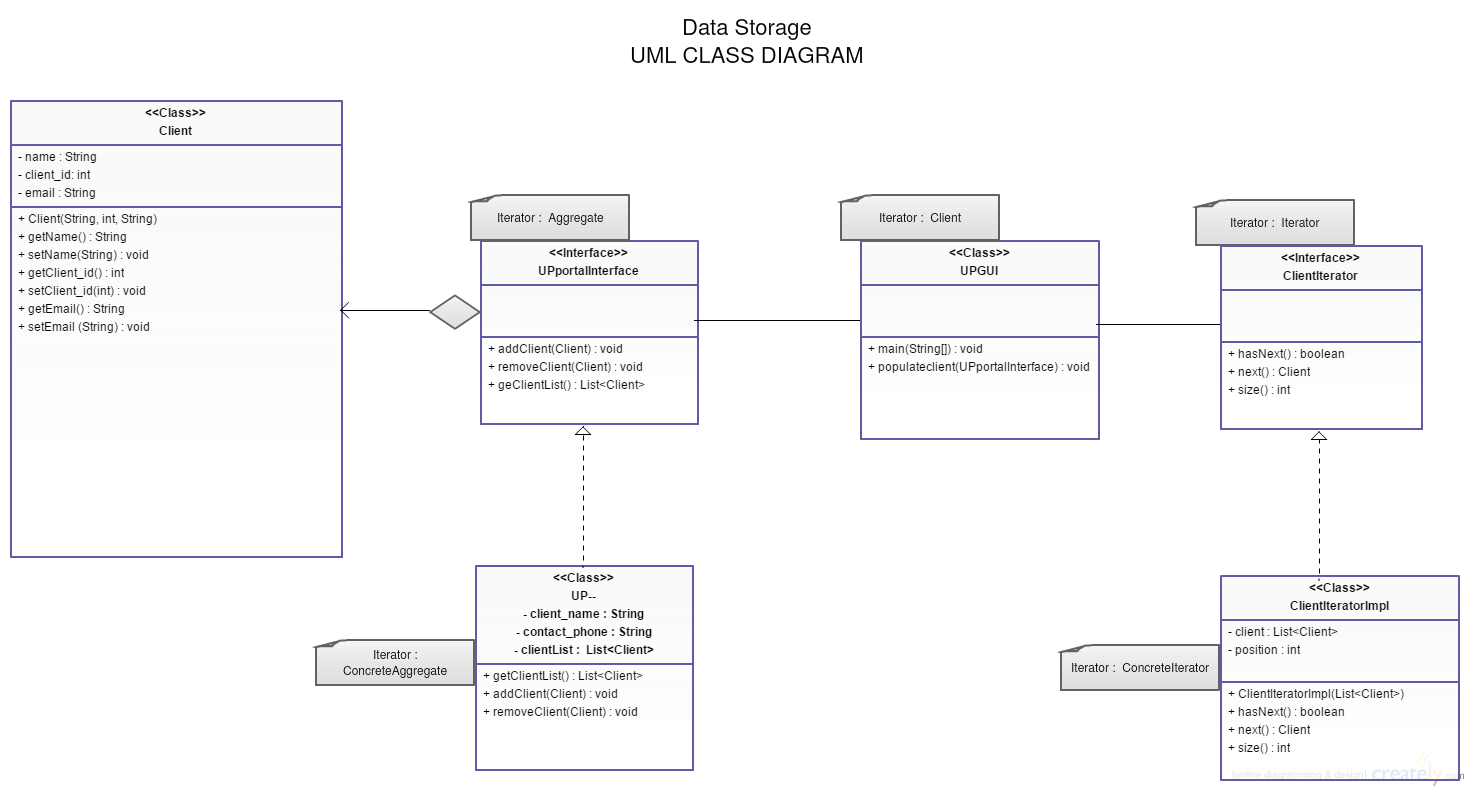
\includegraphics[scale=0.37]{Data-Class-Diagram.png}}}
            \caption{Class Diagram - Data Module}
        \end{figure} 

    % ----- SURVEILLANCE ----- %
    \newpage
    \section{Surveillance}    
        \subsection{Description}    
            The purpose of the surveillance subsystem is to be able to identify locations where there is pedestrian congestion on the walkways of the university.
            By being able to find how many people are connected to the UP routers, which cover a large portion of campus, we are able to more accurately identify these hot-spots and provide this data to the navigation team, in order for people to try avoid these areas. Thus spreading the amount of pedestrians to hopefully avoid highly congested areas. 
        \subsection{Requirements}
        The Surveillance system should be able to:
            \begin{itemize}
                \item Count the number of users connected to a particular router.
                \item Provide a live time data feed of the number of users connected.
                \item Identify the location of each router.
                \item Add or update routers in the system.
                \item Provide loose coupling.
                \item Update the database with information of route congestion in a particular location.
            \end{itemize}
    
        \subsection{Constraints}
        The Surveillance system should operate under the following constraints:
            \begin{itemize}
                \item The list of routers is supplied and assumed to be correct.
                \item Routers are able to connect and receive data from users.
                \item Usernames and passwords for all routers are provided by admins.
            \end{itemize}
        
        \subsection{Design}    
            The surveillance system is implemented using seven classes. We used the mediator design pattern for its implementation.
    
            \subparagraph{Mediator} - The mediator design pattern allows for having two systems (Location and Database) that could then be updated and the same time. \\
            
            This behaviour of this system is important as it allows other modules to also receive a live time feed of every router, but from the database, and not from the surveillance module itself.
            This means that should the surveillance module be taken away no other module would be directly affected and the system would be able to still work. This pattern has therefore allowed us to have low coupling with high cohesion.
    
        \subsection{Implementation Details}    
            To implement the data structure we will use a data structure (linked list, array or vector) to store all the information of the routers and be able to dynamically add to that data structure, while being able to update both data structures on both the database and surveillance module. Way-points which inherit from the locations are  used as the Navigation module has to exist for the program to perform its main purpose, and to avoid duplicating code I inherit from location rather than create a brand new class.

        \begin{figure}[H]
            \centering              
            \centerline{\fbox{\includegraphics[scale=0.35]{Surveillance-Class-Diagram.png}}}
            \caption{Class Diagram - Surveillance Module}
        \end{figure}

        \begin{figure}[H]
            \centering              
            \centerline{\fbox{\includegraphics[scale=0.4]{Surveillance-State-Diagram.png}}}
            \caption{State Diagram - Surveillance Module}
        \end{figure}

        \begin{figure}[H]
            \centering              
            \centerline{\fbox{\includegraphics[scale=0.5]{Surveillance-Case-Diagram.png}}}
            \caption{Use Case Diagram - Surveillance Module}
        \end{figure}  
        
        \begin{figure}[H]
            \centering              
            \centerline{\fbox{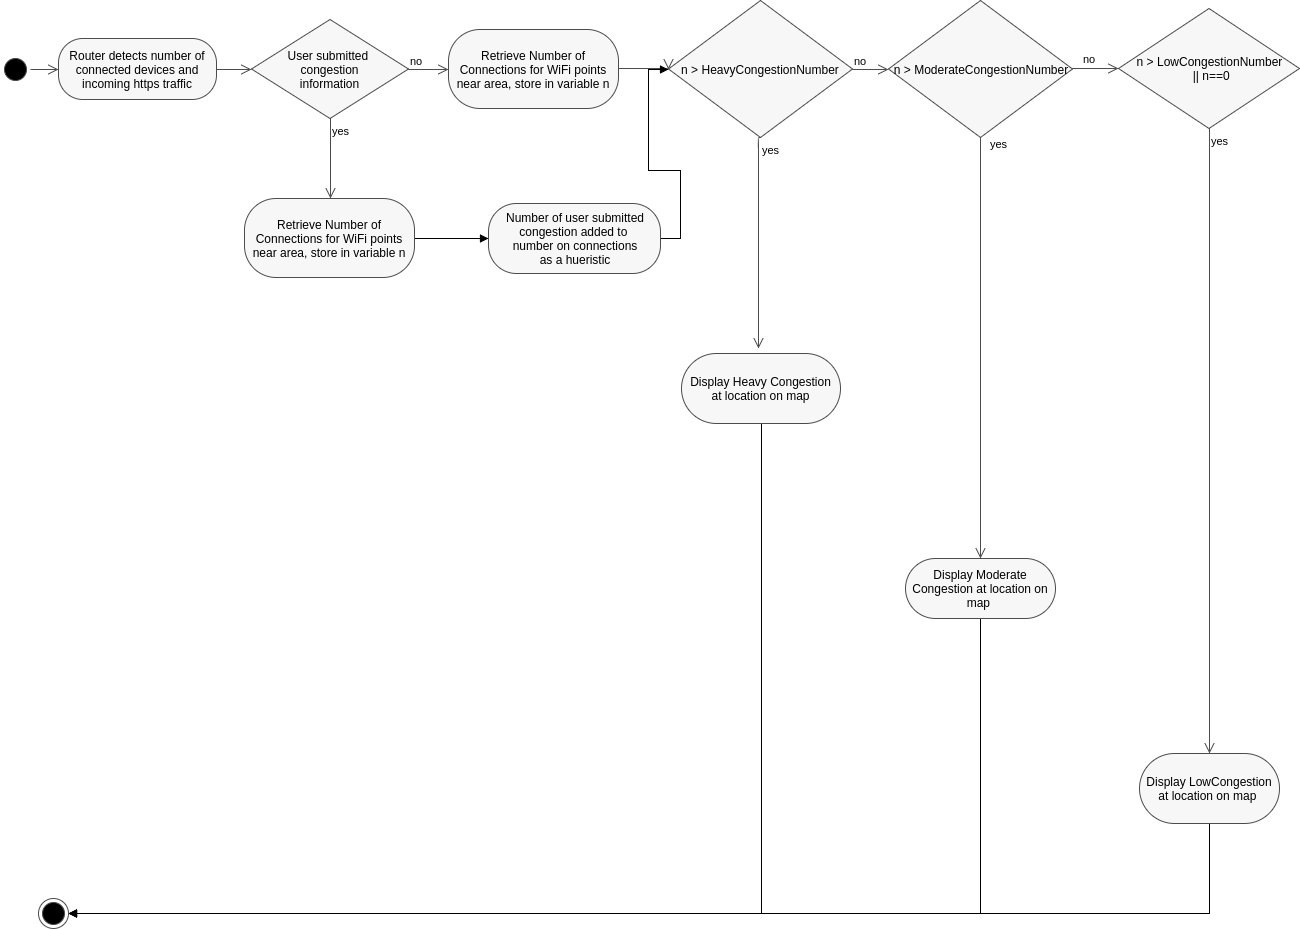
\includegraphics[scale=0.4]{Surveillance-Activity-Diagram.png}}}
            \caption{Activity Diagram - Surveillance Module}
        \end{figure}    
\end{document}
